%************************************************
\chapter{Scheme Design}\label{ch:design}
%************************************************

The purpose of the following section is to describe the solution we propose for enabling usable and secure user authentication, but also to document the analytic work and choices we made in the design process. Based on our general scheme design and user scenarios, we conduct an evaluation of our design and the different benefits it provides.

\section{Design Choices}
\subsection{Learning From Passwords}
The history of authentication schemes has shown, that usability plays a major role in the adoption and practical security of a scheme. During our entire design process, we have carefully aimed to prioritize both usability and security factors, and to continually consider the impact certain design decision may have on the general usability and security of the scheme. 
Given the many problems that currently exist with the widespread use of password-based authentication mechanisms, we envision a solution that is completely free of passwords, and therefore it is not reliant on the knowledge factor, but instead relies on other factors of authentication.

As pointed out by \citet{weirich2001pretty} password reliant schemes have the inherent problem, that users must make a decision between convenience and security when choosing their passwords. This is problematic because users tend to choose convenience in the form of weak passwords, which results in reduced cryptographic strength of the protocol. 
One major benefit of designing a protocol, that does not rely on knowledge factors, is that the individual user no longer chooses a secret that directly impacts the cryptographic strength of the protocol. That being said, it does not mean that a user's behaviour can not directly or indirectly influence the security, of a knowledge-free authentication scheme in other ways. History has shown that attackers will always seek to find the weakest link when finding security vulnerabilities -- so if a protocol is cryptographically sound and strong, it is most likely that an attacker will search for other ways and means to exploit the system.

\subsection{Transparency}
We seek to design a transparent authentication scheme, that reduces the user's direct involvement in the task of authentication, and instead performs most of the work in the background. This idea is grounded in the theory by \citet{weirich2001pretty}, which states that users consider the act of authentication to be an enabling task, that should be quick and effective, to get to the primary task. Thus if it is possible to design a scheme such that the authentication process can be done securely and efficiently, while at the same time being unobtrusive to the user, it will be ideal, since it enables users to reach their primary tasks quicker and with less effort.

In previous work \cite{bianchi2016wearable, ceccarelli2015continuous, ojala2008wearable} the term `transparent login' or `transparent authentication' is used to describe authentication systems where little or no user interaction is required to perform authentication, and thus the whole process is being `transparent' to the user because it happens in the background. The meaning of the term `transparent', in this context, suggests that the authentication process is hidden or even invisible to the user. We consider the term `transparent' to be rather ambiguous, since it could be interpreted as something that is easy to understand and without secrets. The Oxford English Dictionary definition of the word `transparent' also indicate different interpretations; In a general context: \textit{Easy to perceive or detect}, and in a computing context: \textit{Functioning without the user being aware of its presence}.

%\begin{enumerate*}
%    \item[1)] In a general context: \textit{East to perceive or detect}, 
%    \item[2) In a computing context: \textit{Functioning without the user being aware of its presence}.
%\end{enumerate*}

%In general context: \textit{``Easy to perceive or detect.''}.
%In computing context:\textit{ ``(of a process or interface) functioning without the user being aware of its presence.''.}

To clarify -- when we say we want to design a transparent authentication scheme, we adopt the meaning from previous work \cite{bianchi2016wearable, ceccarelli2015continuous, ojala2008wearable}, to the extent that user interaction should be implicit, and that the authentication process happens in the background. However, we also include the other aspect of the word `transparent' in our definition, meaning that the actions of the system must be easily perceivable for users. This concept is more precisely expressed by \citet{bellotti2001intelligibility}, who uses the term `intelligibility' to describe a system's ability to present to its users what it knows, how it knows it, and what it will do with its knowledge. They point out the importance of user involvement and `intelligibility' in context-aware systems, if a system's behaviour must be acceptable to its users. While our authentication system may not be classifiable as context-aware, it will take partially autonomous actions, without a user's explicit instructions, in the same manner as context-aware systems do. 
In summary, we consider intelligibility as an important factor, and thus define `transparent authentication' as an authentication process that is without any user interaction, but with the user's awareness of when and where he is authenticated, even though he might not be an active participant. The user must never be in doubt of, whether or not, he is currently authenticated at some service or device -- should he want to have this information. 

\subsection{Adjustable User Awareness and Explicit Consent}
We want to design our scheme, such that different levels of security can be used, depending on the requirement of the particular use case. Specifically, it should be possible in some cases, to increase the amount of user awareness of what is happening transparently, for instance in the form of event notifications given to the user. In some cases, the user might even be required to explicitly give his consent to authentication requests and transactions.
This, of course, implies a reduction in the unobtrusiveness of the scheme from the users perspective, but can potentially provide increased certainty that no adversary is misusing the transparent mechanisms of the scheme, to gain access without the user noticing. We argue that this cost is acceptable in some situations. For instance, it is easy to imagine that users want an extra degree of security for their online banking accounts and for performing money transfers compared to viewing their news feed on a social media account. 
Thus our scheme should support different levels of user awareness and explicit consent, that can be adjusted based on users and service providers preferences. 

\begin{figure}[hb]
    \centering
    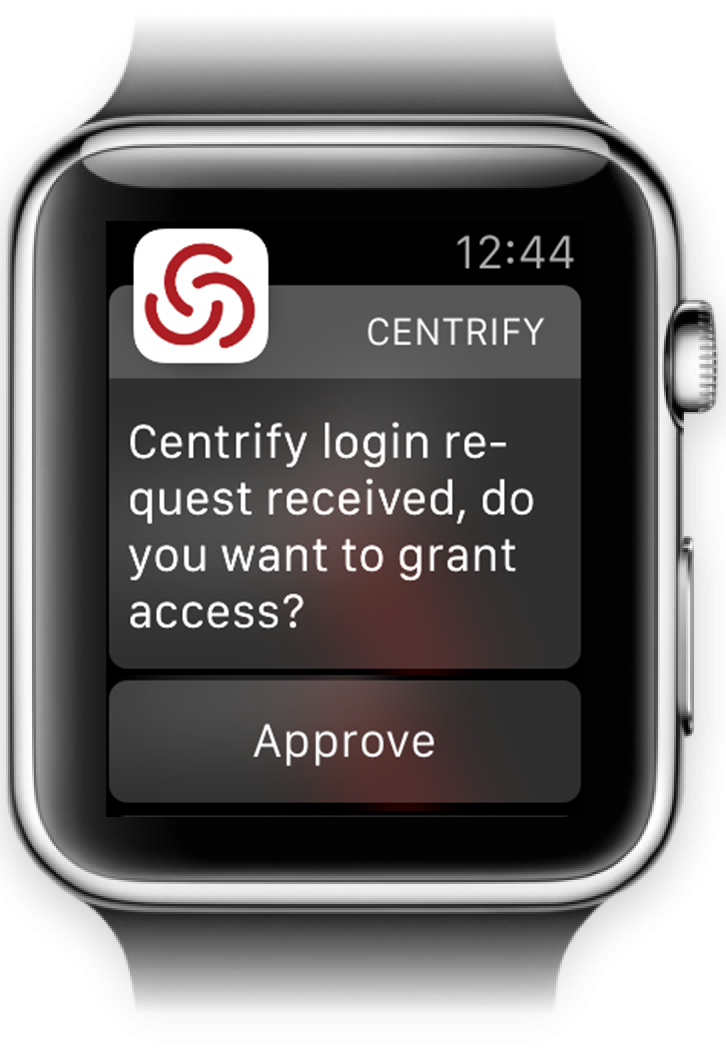
\includegraphics[width=.35\linewidth]{gfx/consent}
    \caption{Example of Explicit User Consent}
\end{figure}

\subsection{Why Wearables?}
\fquotet{A general trend is clear: wearables provide novel opportunities \\ to improve or re- design approaches to authentication.}{bianchi2016wearable}
\bigskip

\citet{ojala2008wearable} used an approach with wearable authentication in their proposed scheme. Their solution was a custom built wearable wristband with different sensors and a computer attached, which was highly specialized to be used for authentication only. 
Within recent years wearable computing devices (commonly referred to as 'wearables') has become available to the end-user market, intended for multi-purpose use, and not for authentication only. These recent advances have made wearables regain the attention from security researchers, to explore the different opportunities that wearables can provide for user authentication \cite{bianchi2016wearable}. 
We want our authentication scheme to utilize wearables, for several reasons. First, the many sensors embedded into wearables provide an easy way to harvest input data implicitly about the wearing user. Furthermore many wearable devices come with light sensors that can report when a user is wearing the device or have taken it off. In short, the embedded sensors can help to establish more confidence in a user's identity, which is very useful for providing secure authentication. Second, the processing power and network capabilities of wearables have grown, now enabling them to run authentication mechanisms based on strong cryptography. Third, the use of wearables allows our protocol to run on commodity hardware, that is already widely known and used, thus allowing us to focus less on hardware details of the scheme, and at the same time increasing the chance that users will adopt the system, if they already own the required hardware. 

\subsection{Proximity}
In order to provide transparent authentication, some mechanisms must be put in place to autonomously decide when and where authentication should take place, whenever the user is not directly involved in the process. Taking inspiration from both \citet{bardram2003context} and \citet{ojala2008wearable} we want the authentication scheme to be proximity-based. Ideally, a user should be able to walk up to a computer and as soon as he is within a specified range, the transparent authentication process should initiate. To do this a user must carry a wearable device that is capable of providing evidence of the user's identity, to client computers where the user wants to authenticate at. We imagine that the Bluetooth protocol would be an ideal solution to support proximity-based authentication between the wearable devices and the client computers. While it may be an implementation detail, Bluetooth is to a large extend the communication standard that what we have had in mind when we designed our scheme. Additionally, the choice of a widely used communication standard as Bluetooth also aligns well with our choice of wearables, and the preference of mature commodity technologies over highly specialized solutions.

\subsection{Continuity}

When making the authentication mechanism more transparent (unobtrusive), a problem might be that the user is not aware that he is authenticated with the system that he is using (even if the information is available to him, he might overlook the fact), and thus walk away from an active session. 

\fquotet{During our experiments we discovered that the process of logging out a user is equally important. [...] Although this is normally not considered to be part of a user authentication mechanism, we argue that logout has to be considered as a part of the design as well.}{bardram2003context}

Continuous authentication entails verification of user identity on an ongoing basis during an authentication session, thus greatly increasing the certainty that only the legitimate user is accessing protected resources~\cite{ojala2008wearable}. A problem with many services today, is that clients are allowed to store user credentials or save access tokens without expiration in cookies, such that no confirmation of the user's identity is done after initial verification. This design is needed to reduce constant user interaction, because of the heavy reliance of password in current schemes. However this comes with the trade-off, that a non legitimate user can access private resources, in case of theft or loss of a device. 

We found that continuous authentication synergises well with prox\-imity-based, transparent and wearable authentication. 
Since we are using a transparent authentication scheme we do not need to store login information on the client, since the information needed to verify a user's identity, can be acquired without interrupting the user, even if it is done very frequently. After a user has established initial authentication, we can continually confirm that the basic requirements for authentication are still met, such as the user having to wear the wearable device actively, and be within proximity of the client he is authenticated at.

It is important to mention that literature uses the term `continuous' differently. It can either describe the process of continuous verification to keep an authenticator unlocked (as in the case of the Pico~\cite{stajano2011pico}), or be a continuous verification process with a verifier (as in the case of Wearable Auth~\cite{ojala2008wearable}). We aim to include \textit{both} aspects.

\subsection{Authenticator and Sibling}
In order to make our scheme more resilient to theft or loss of the wearable device, and also less vulnerable in case the device is compromised, the scheme is designed to be used with an additional device, that works together with the wearable device to decide whether authentication is allowed or not. If an attacker gains access (physically or virtually), to one of the devices, but not both, it should not be possible to achieve any successful attacks. We have designed it such that the device pair, form a master/slave relationship, where outside parties communicate only with the master device to request authentication access. We generally refer to the two devices as the \gls{authenticator} acting as the master and the \gls{sibling} acting as the slave device. Loosely defined the \gls{authenticator} could be any type of computational device. Table~\ref{table:device_table} shows the requirements for the two devices. 

\begin{table}[bth]
\centering
\vspace{8em}
%\resizebox{\linewidth}{!}{
% \setlength\tabcolsep{1.8pt}
\begin{tabular}{r|ccccccc}
& \begin{rotate}{55}\textit{Being worn by a user}\end{rotate}
& \begin{rotate}{55}\textit{Verifying a users identity}\end{rotate}
& \begin{rotate}{55}\textit{Monitoring if worn}\end{rotate}
& \begin{rotate}{55}\textit{Receiving basic user-input}\end{rotate}
& \begin{rotate}{55}\textit{Displaying messages}\end{rotate}
& \begin{rotate}{55}\textit{Cryptographic computations}\end{rotate}
& \begin{rotate}{55}\textit{Bluetooth LTE I/O} \end{rotate} \\ \hline

Authenticator &
\CIRCLE &
\CIRCLE &
\CIRCLE &
\CIRCLE &
\CIRCLE &
\CIRCLE &
\CIRCLE \\ \hline
Sibling &
&
&
&
&
&
\CIRCLE &
\CIRCLE \\ \hline

    \end{tabular}
%}
\caption[Overview of device requirements]{The requirements of devices used as authenticators and siblings.}
\label{table:device_table}
\end{table}

\begin{comment}
\begin{itemize}
    \item Being worn by a user
    \item Verifying a users identity
    \item Monitoring when it is worn and when it is taken off
    \item Receiving basic input from user
    \item Displaying output messages
    \item Performing basic cryptographic computations 
    \item Sending/receiving data over Bluetooth
\end{itemize}

The \gls{sibling} has fewer requirements. It can be any type of computational device, as long as it is capable of:
  
\begin{itemize}
    \item Performing basic cryptographic computations 
    \item Sending/receiving data over Bluetooth
\end{itemize}
\end{comment}

While we claim that our scheme design and concepts of \gls{authenticator} and \gls{sibling} are not locked to a specific device type, we have primarily considered and worked with the case of a smartwatch as \gls{authenticator} and a smartphone as \gls{sibling}. We will therefore not rule out completely, that certain design choices have been made with these two device types in mind. The main reason for this is to use devices that the user will already carry around with him. Although wearables are not so common yet, they are slowly getting traction. By using devices that the user already has in his vicinity, we increase the transparency of the solution, both in terms of the user not needing to remember bringing a dedicated authentication device, and in terms of hiding the solution in devices, he already carries around.

%\todo[inline]{We need to change this part. The main argument should be that it is devices that the user (likely) already owns and carries around.}

%The reason for choosing a smartwatch and smartphone, is that in addition to each fulfilling all the basic requirements listed above, they are both easy to work and experiment with from a prototyping perspective. This has allowed us to focus on scheme design and core functionality, and not hardware/software issues related to the platform.
%Another benefit is that both device types are widely available and recognized as consumer products, which makes it more easy for readers of this thesis to relate to, and understand how they could be used in practice. 


\section{The Scheme in Practice} \label{sec:scheme_desc}
The design choices above, lead us to the following more brief and concrete description of how our authentication scheme should work in practice:

The scheme involves 4 different communicating parties. The \gls{authenticator}, the \gls{sibling}, the \gls{client} and the \gls{server}. A user carries two personal physical devices: the \gls{authenticator} and the \gls{sibling}, which are a smartwatch and a smartphone respectively. The \gls{authenticator} acts as a key which is unique to each user and required for authentication. However the \gls{authenticator} should only allow authentication if it is actively worn by the user, and in proximity of its \gls{sibling} device. If at any time the user takes off the \gls{authenticator} from his wrist, or if the \gls{sibling} is not nearby, the \gls{authenticator} should go into \textbf{locked} state, effectively meaning that all authentication requests it receives are denied. Furthermore, the \gls{authenticator} should return to \textbf{unlocked} state once the \gls{sibling} is again within proximity, or if the user re-equips the \gls{authenticator} on his wrist and reconfirms his identity, either by using biometric sensors, pin code or some other mechanism available from the \gls{authenticator}.  

The user interacts with a \gls{client} which is the device from where the authentication process is initiated. A \gls{client} could for instance be a laptop or desktop computer, which is used to login to some online service, that requires authentication. 

The \gls{client} is not an active participant in the authentication process. Rather, when the user tries to authenticate with a \gls{server} through the \gls{client}, and the \gls{authenticator} is nearby and \textbf{unlocked}, then the \gls{authenticator} will be required to provide evidence of the identity.
If the evidence is accepted by the \gls{server}, then the \gls{client} is authenticated.

%The \gls{client} is not directly handling authentication but merely contacts a \gls{server} that owns some protected resources. The \gls{server} requires the \gls{client} to prove that the \gls{authenticator} is indeed in range of the \gls{client} and is worn by the user, in order to allow access to its resources. Thus the main responsibility of the \gls{client} is to serve content, and act as a middle man for communication between the \gls{authenticator} and the \gls{server}.

The scheme is backed by a protocol that continually authenticates the user as long as the \gls{authenticator} is worn in close range of the \gls{client} and in \textbf{unlocked} state. If one of the conditions are not met at any time, the authentication session should terminate.

\begin{figure}
  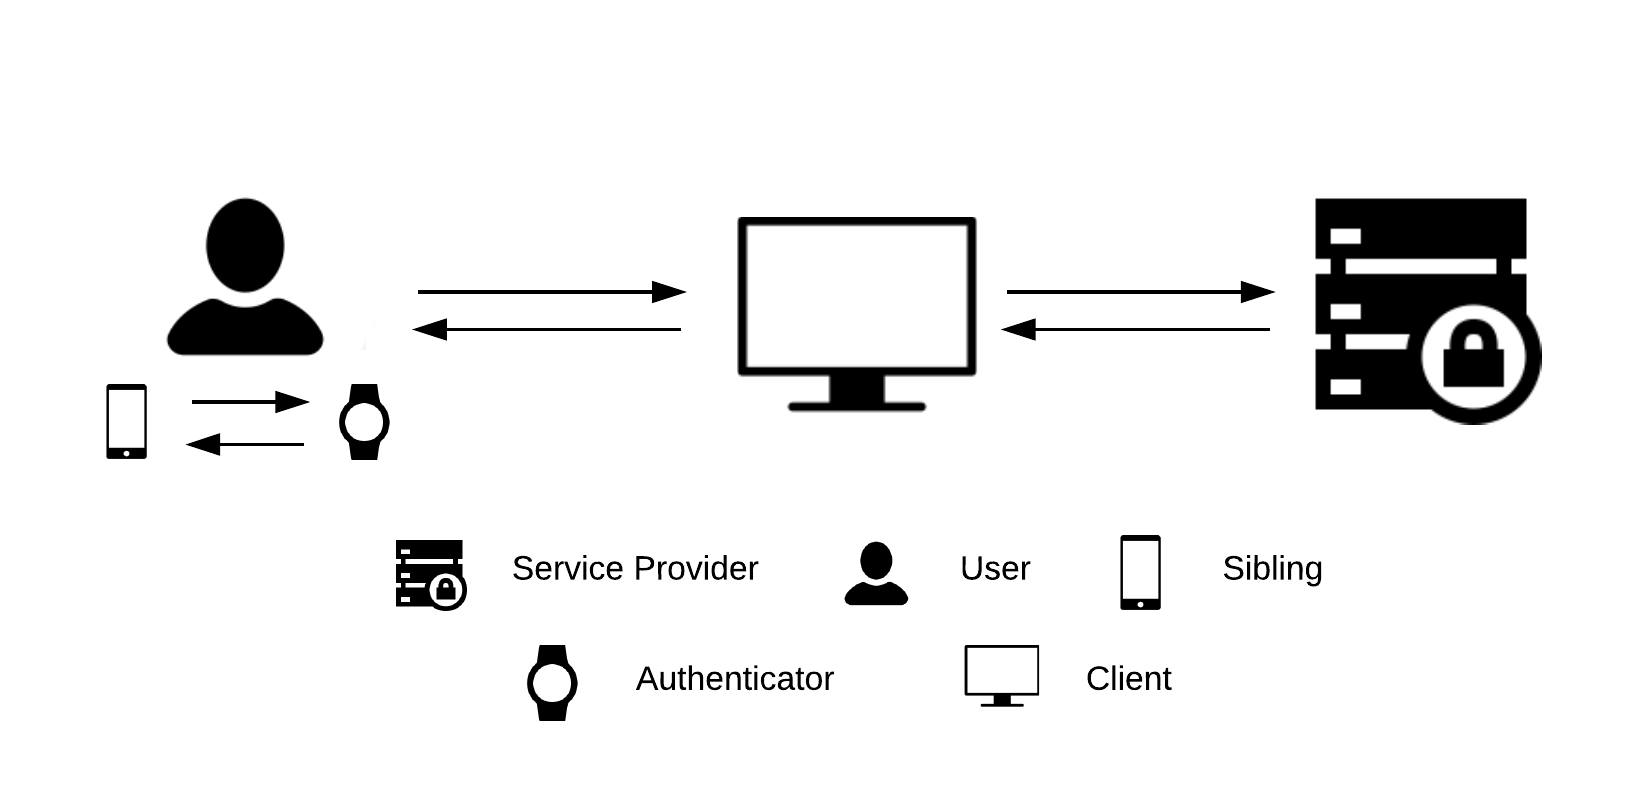
\includegraphics[width=\linewidth]{gfx/scheme_diagram.png}
  \caption{Component overview for the propose scheme}
  \label{fig:scheme_diagram}
\end{figure}


\section{User Scenarios} \label{sec:scenarios}
Below we describe 4 different user scenarios for our authentication scheme. The scenarios describe the most commonly occurring situations in the use of our proposed scheme. The intention of these scenarios is to gain insight into how the user interacts with the system, and to demonstrate which problems it solves for the user. 
The different actors appearing across the scenarios are the same as presented above in \ref{sec:scheme_desc}: \gls{authenticator}, \gls{sibling}, \gls{client} and \gls{server}. We differentiate between two levels of user involvement, where \gls{awareness} is the least obtrusive of the two:
\begin{itemize}
    \item[] \Gls{awareness}: \textit{The user is notified about important events, but does not require the user to actively perform any actions.}
    \item[] \Gls{exp_consent}: \textit{The user is required to actively perform an action, typically in the form of accepting/denying certain requests between the involved actors.}
\end{itemize}

The scenarios are listed in table~\ref{sc:register}, \ref{sc:unlocking}, \ref{sc:auth}, and \ref{sc:theft}.



\begin{scenario}{Registration with a Service Provider}{Scenario: Registration}{register}
    \row{Actors}{\gls{authenticator} $A$, \gls{client} $C$, \gls{server} $S$}
    \row{User involvement}{Awareness, optional:Explicit consent}
    \row{Authenticator State}{$unlocked$}
    \row{Description}{A user wants to register for a service $S$ and uses a \gls{client} $C$ to send a registration request to $S$. $S$ now communicates with the users \gls{authenticator} $A$ through $C$ and asks for confirmation of the registration. $A$ now notifies the user and optionally ask the user to confirm the registration request, before sending back needed information to $S$ to complete the registration process.}
\end{scenario}

\begin{scenario}{Unlocking the Authenticator}{Scenario: Unlocking}{unlocking}
    \row{Actors}{\gls{authenticator} $A$, \gls{sibling} $As$}
    \row{User involvement}{Awareness, optional:Explicit consent}
    \row{Authenticator State}{$locked \Rightarrow unlocked$}
    \row{Description}{A users watch acting as \gls{authenticator} $A$ is $locked$ and he wishes to unlock it. The user puts on the watch, which registers that it has been put on by its owner, and starts monitoring that it remains attached. $A$ now communicates with its sibling $As$, and asks for permission to unlock. After an optional user interaction with $As$, it communicates back with an acknowledgement, that allows $A$ to unlock. $A$ now notifies the user that it is $unlocked$. $A$ remains $unlocked$ for as long it is attached to the users wrist, and in range of $As$.}
\end{scenario}

\begin{scenario}{Establishing a Session}{Scenario: Authentication}{auth}
    \row{Actors}{\gls{authenticator} $A$, \gls{client} $C$, \gls{server} $S$}
    \row{User involvement}{Awareness, optional:Explicit consent}
    \row{Authenticator State}{$unlocked$}
    \row{Description}{A user wants to establish a session with a \gls{server} $S$ through a \gls{client} $C$. $S$ replies with a challenge, which requires $C$ to prove that it is a legitimate user who is requesting access. $C$ forwards the challenge to the users nearby \gls{authenticator} $A$, which is currently $unlocked$. $A$ optionally asks the user to confirm the authentication request, and then replies back with a response to the challenge generated by $S$. $C$ now sends the challenge response back to $S$, and if $S$ accepts the solution to the challenge, then an authentication sessions is established. $A$ notifies the user that the sessions is established. If the session is not explicitly cancelled by the user, the session is maintained as long as $A$ remains unlocked and $A$ remains in proximity of $C$.}
\end{scenario}

\begin{scenario}{Theft or Loss}{Scenario: Theft or loss}{theft}
    \row{Actors}{\gls{authenticator} $A$, \gls{sibling} $As$}
    \row{User involvement}{Explicit consent}
    \row{Authenticator State}{$unlocked \lor locked \Rightarrow lockdown$}
    \row{Description}{A user notices that either his \gls{authenticator} $A$ or \gls{sibling} $As$ is missing. The user uses the remaining device to activate $lockdown$. In this state $A$ can no longer be unlocked (even when in proximity of $As$), and therefore not authenticate with any services. The $lockdown$ state remains until a recovery procedure has taken place, either if the missing device resurfaces, or if a new device is used for recovery.}
\end{scenario}


\section{Scheme Evaluation}

In this section we evaluate our proposed authentication scheme, in comparison to the review in chapter~\ref{ch:review}. In addition to the benefits defined by the framework, we define four new properties, that we based on our analysis consider equally relevant for authentication. An overview is shown in table~\ref{table:property_table}.



\subsection{Extending the Evaluation Framework}\label{sec:extending_framework}
We extend the framework \cite{bonneau2012quest}, with 2 usability properties: \textit{Awareness} and \textit{No-Config}; and 2 security properties: \textit{No-Intermediary-Knowledge} and \textit{Continuous}. 

\paragraph{Awareness:} The scheme can make its users aware of its current state, and the decisions it takes autonomously. We grant \textit{Awareness} if a user of the scheme is capable of knowing where he is currently authenticating/authenticated at, at all times. This benefit is considered important from a usability perspective, since it helps a user to understand what happens transparently, and avoid undesirable situations as where a user think he is authenticated but actually is not, and conversely actually is authenticated, but think he is not.
    
\paragraph{No-Config:} We award \textit{No-Config} if the act of authentication or user registration does not require any additional configuration steps the first time a specific client is used by a specific user, compared to if the client was used previously by the specific user. 
Thus a user must be able to walk up to any arbitrary client and use the scheme for authentication or registration, with the same amount of required effort, as on a client where he has used the scheme, several times before. Note that \textit{No-Config} does not mean that no initial configuration might be needed on a client in order to run the scheme (eg. installing a browser plugin or enabling Bluetooth). Rather it means that no additional configuration is required specifically because it is a new user of the client. Password managers are a type of scheme that typically does not offer this benefit, since a user will have to undergo an extra step the first time he uses a new client in order to transfer his keychain onto it. The benefit of \textit{No-Config} is considered a usability benefit, because it reduces the time a user has to spend on authentication the first time he uses a new client. It is especially important in environments where many public computers are used, and a user does not have a personal computer.
    
\paragraph{No-Intermediary-Knowledge:} During authentication or registration the client is not exposed to any information with long-term value. We grant \textit{No-Intermediary-Knowledge} if no secrets (such as passwords), that could be used to authenticate at a later point in time, is given or inputted on the client. \textit{No-Intermediary-Knowledge} is a security benefit and is considered important because it limits the power of an adversary in full or partial control of the client.
    
\paragraph{Continuous:} The scheme supports continuous authentication. We grant the benefit if a scheme reconfirms a user's identity with a verifier regularly after initial authentication, and is capable of stopping the authentication session whenever the user's identity can not be verified any longer. This benefit is a security benefit, and limits the power of an adversary with physical or remote access to a client greatly, since the authentication sessions are not kept alive for an extended duration after the user is no longer actively engaged.

We grant \textit{Quasi-Continuous} if the system is using a hardware token and only the token is continuously authenticated, but sessions with services are not.

\subsection{Rating Process} \label{sec:rating_process}
The authentication scheme proposed in this thesis is intended as an improvement over password. It aims to improve security and usability of passwords, but does not aim to surpass passwords in terms of deployability.

The scheme is \textit{Memorywise-Effortless} by design because it is a transparent authentication scheme, and therefore does not require the user to input anything from memory or perform some memorized interaction in order to authenticate. For the same reasons and since no new hardware has to be introduced to the user, we award \textit{Easy-to-learn}. The proximity-based login approach of the scheme ensures that it is \textit{Physically-Effortless} to use, as the only real physical requirements of the user to use the scheme for authentication, is that the user must wear a watch and carry a phone, and move within close range of the client where authentication is performed at. 

We grant \textit{Efficient-to-Use} and \textit{Infrequent-Errors} because the scheme is designed to have minor user interaction, and the cryptographic exchanges between \gls{server} and \gls{authenticator}, is carried out much faster than the time taken for typing even a simple password. Furthermore, the scheme does not rely on biometrics or other methods of authentication that could introduce false-negatives. The scheme is \textit{Scalable-for-Users}, as an increased number of links between users and \glspl{server} does not have any impact on the individual users experience. We award the scheme \textit{Quasi-Nothing-to-Carry}, because the benefit can only be granted if the user has to carry nothing at all. However, if the devices are considered something which the user always carry around anyway, in this case, a phone and a watch, the applied burden on the user is arguably reduced significantly. We do not grant the scheme \textit{Easy-Recovery-from-Loss} since no such mechanism exists for the scheme in its current design state. 
We grant \textit{Awareness} as the scheme is designed to send notifications to a user on his watch, whenever a new registration or authentication session is started. The scheme does not offer the benefit of \textit{No-Config} as a pairing process is required between \gls{client} and \gls{authenticator}, the first time a new \gls{client} is used. 

\begin{table}[bth]
\centering
\begin{wide}
\resizebox{\linewidth}{!}{
%\rotatebox{270}{
\setlength\tabcolsep{1.8pt}
\begin{tabular}{r|c|cccccccccc|cccccc|ccccccccccccc}

\multicolumn{2}{c}{} &
\multicolumn{10}{c}{\textbf{Usability}} &
\multicolumn{6}{c}{\textbf{Deployability}} &
\multicolumn{13}{c}{\textbf{Security}}\\
\multicolumn{31}{c}{}
\\

& \rot{\textit{Reference}} &
\rot{\textit{Memorywise-Effortless}} &
\rot{\textit{Scalable-for-Users}} &
\rot{\textit{Nothing-to-Carry}} &
\rot{\textit{Physically-Effortless}} &
\rot{\textit{Easy-to-Learn}} &
\rot{\textit{Efficient-to-Use}} &
\rot{\textit{Infrequent-Errors}} &
\rot{\textit{Easy-Recovery-from-Loss}} &
\rot{\textit{Awareness}} &
% \rot{\textit{Multi-User-Support}} &
\rot{\textit{No-Config}} &
\rot{\textit{Accessible}} &
\rot{\textit{Negligible-Cost-per-User}} &
\rot{\textit{Server-Compatible}} &
\rot{\textit{Browser-Compatible}} &
\rot{\textit{Mature}} &
\rot{\textit{Non-Proprietary}} &
\rot{\textit{Resilient-to-Physical-Observation}} &
\rot{\textit{Resilient-to-Targeted-Impersonation}} &
\rot{\textit{Resilient-to-Throttled-Guessing}} &
\rot{\textit{Resilient-to-Unthrottled-Guessing}} &
\rot{\textit{Resilient-to-Internal-Observation}} &
\rot{\textit{Resilient-to-Leaks-from-Other-Verifiers}} &
\rot{\textit{Resilient-to-Phishing}} &
\rot{\textit{Resilient-to-Theft}} &
\rot{\textit{No-Trusted-Third-Party}} &
\rot{\textit{Requiring-Explicit-Consent}} &
\rot{\textit{Unlinkable}} &
\rot{\textit{No-Intermediary-Knowledge}} &
\rot{\textit{Continuous}} \\ \hline

Passwords & &
            & %Memorywise-Effortless
            & %Scalable-for-Users
\CIRCLE     & %Nothing-to-Carry
            & %Physically-Effortless
\CIRCLE     & %Easy-to-Learn
\CIRCLE     & %Efficient-to-Use
\Circle     & %Infrequent-Errors
\CIRCLE     & %Easy-Recovery-from-Loss
            & %Awareness
%           & %Multi-User-Support
\CIRCLE     & %No-Pairing
\CIRCLE     & %Accessible
\CIRCLE     & %Neglible-Cost-per-User
\CIRCLE     & %Server-Compatible
\CIRCLE     & %Browser-Compatible
\CIRCLE     & %Mature
\CIRCLE     & %Non-Proprietary
            & %Resilient-to-Physical-Observation
\Circle     & %Resilient-to-Targeted-Impersonation
            & %Resilient-to-Throttled-Guessing
            & %Resilient-to-Unthrottled-Guessing
            & %Resilient-to-Internal-Observation
            & %Resilient-to-Leaks-from-Other-Verifiers
            & %Resilient-to-Phishing
\CIRCLE     & %Resilient-to-Theft
\CIRCLE     & %No-Trusted-Third-Party
\CIRCLE     & %Requiring-Explicit-Consent
\CIRCLE     & %Unlinkable
            & %No-Intermediary-Knowledge
              %Continuous
\\ \hline

Context-Aware Auth~~& \cite{bardram2003context} &
\Circle     & %Memorywise-Effortless
\CIRCLE     & %Scalable-for-Users
            & %Nothing-to-Carry
\Circle     & %Physically-Effortless
\CIRCLE     & %Easy-to-Learn
\CIRCLE     & %Efficient-to-Use
\CIRCLE     & %Infrequent-Errors
            & %Easy-Recovery-from-Loss
            & %Awareness
%           & %Multi-User-Support
\CIRCLE     & %No-Pairing
\CIRCLE     & %Accessible
            & %Neglible-Cost-per-User
            & %Server-Compatible
            & %Browser-Compatible
            & %Mature
\CIRCLE     & %Non-Proprietary
\Circle     & %Resilient-to-Physical-Observation
\CIRCLE     & %Resilient-to-Targeted-Impersonation
            & %Resilient-to-Throttled-Guessing
            & %Resilient-to-Unthrottled-Guessing
\Circle     & %Resilient-to-Internal-Observation
            & %Resilient-to-Leaks-from-Other-Verifiers
\Circle     & %Resilient-to-Phishing
\Circle     & %Resilient-to-Theft
            & %No-Trusted-Third-Party
\CIRCLE     & %Requiring-Explicit-Consent
            & %Unlinkable
\Circle     & %No-Intermediary-Knowledge
\Circle       %Continuous
\\ \hline

Wearable Auth & \cite{ojala2008wearable} &
\CIRCLE     & %Memorywise-Effortless
\CIRCLE     & %Scalable-for-Users
\Circle     & %Nothing-to-Carry
\Circle     & %Physically-Effortless
\CIRCLE     & %Easy-to-Learn
\CIRCLE     & %Efficient-to-Use
\CIRCLE     & %Infrequent-Errors
            & %Easy-Recovery-from-Loss
            & %Awareness
%           & %Multi-User-Support
            & %No-Pairing
\CIRCLE     & %Accessible
            & %Neglible-Cost-per-User
            & %Server-Compatible
            & %Browser-Compatible
            & %Mature
\CIRCLE     & %Non-Proprietary
\CIRCLE     & %Resilient-to-Physical-Observation
\CIRCLE     & %Resilient-to-Targeted-Impersonation
\CIRCLE     & %Resilient-to-Throttled-Guessing
\CIRCLE     & %Resilient-to-Unthrottled-Guessing
?           & %Resilient-to-Internal-Observation
?           & %Resilient-to-Leaks-from-Other-Verifiers
\CIRCLE     & %Resilient-to-Phishing
\CIRCLE     & %Resilient-to-Theft
?           & %No-Trusted-Third-Party
\Circle     & %Requiring-Explicit-Consent
?           & %Unlinkable
?           & %No-Intermediary-Knowledge
\CIRCLE       %Continuous
\\ \hline

Pico & \cite{stajano2011pico} &
\CIRCLE     & %Memorywise-Effortless
\CIRCLE     & %Scalable-for-Users
            & %Nothing-to-Carry
\CIRCLE     & %Physically-Effortless
            & %Easy-to-Learn
\Circle     & %Efficient-to-Use
\Circle     & %Infrequent-Errors
            & %Easy-Recovery-from-Loss
            & %Awareness
%           & %Multi-User-Support
            & %No-Pairing
            & %Accessible
            & %Neglible-Cost-per-User
            & %Server-Compatible
            & %Browser-Compatible
            & %Mature
\CIRCLE     & %Non-Proprietary
\CIRCLE     & %Resilient-to-Physical-Observation
\CIRCLE     & %Resilient-to-Targeted-Impersonation
\CIRCLE     & %Resilient-to-Throttled-Guessing
\CIRCLE     & %Resilient-to-Unthrottled-Guessing
\CIRCLE     & %Resilient-to-Internal-Observation
\CIRCLE     & %Resilient-to-Leaks-from-Other-Verifiers
\CIRCLE     & %Resilient-to-Phishing
\Circle     & %Resilient-to-Theft
\CIRCLE     & %No-Trusted-Third-Party
\CIRCLE     & %Requiring-Explicit-Consent
\CIRCLE     & %Unlinkable
\CIRCLE     & %No-Intermediary-Knowledge
\Circle       %Continuous
\\ \hline

Our design & &
\CIRCLE     & %Memorywise-Effortless
\CIRCLE     & %Scalable-for-Users
\Circle     & %Nothing-to-Carry
\CIRCLE     & %Physically-Effortless
\CIRCLE     & %Easy-to-Learn
\CIRCLE     & %Efficient-to-Use
\CIRCLE     & %Infrequent-Errors
            & %Easy-Recovery-from-Loss
\CIRCLE     & %Awareness
%           & %Multi-User-Support
            & %No-Pairing
\CIRCLE     & %Accessible
\Circle     & %Neglible-Cost-per-User
            & %Server-Compatible
            & %Browser-Compatible
            & %Mature
\CIRCLE     & %Non-Proprietary
\CIRCLE     & %Resilient-to-Physical-Observation
\CIRCLE     & %Resilient-to-Targeted-Impersonation
\CIRCLE     & %Resilient-to-Throttled-Guessing
\CIRCLE     & %Resilient-to-Unthrottled-Guessing
\Circle     & %Resilient-to-Internal-Observation
\CIRCLE     & %Resilient-to-Leaks-from-Other-Verifiers
\CIRCLE     & %Resilient-to-Phishing
\Circle     & %Resilient-to-Theft
\CIRCLE     & %No-Trusted-Third-Party
\Circle     & %Requiring-Explicit-Consent
\CIRCLE     & %Unlinkable
\CIRCLE     & %No-Intermediary-Knowledge
\CIRCLE       %Continuous
\\ \hline
\multicolumn{31}{r}{

\CIRCLE~=~offers the benefit 
\quad \Circle~=~almost offers the benefit
%\quad \textit{no circle}~=~does not offer the benefit 
\quad ?~=~not known}
\quad \\

\end{tabular}}
\end{wide}

\caption[Overview of benefits of our design]{Comparing the benefits of passwords with related work in Pervasive Authentication and the (envisioned) benefits of our design.}
\label{table:property_table}
\end{table}

The scheme is \textit{Accessible} since no physically constraining activities are involved in the use of the scheme. We grant it \textit{Quasi-Negligible-Cost-per-User}, as the required devices: smartphone and smartwatch, are relatively costly on one hand, but on the other hand is something that can be used for many other purposes and is already owned by many users.
As the scheme aims to be a complete password replacement, it is not designed to prioritize \textit{Server-Compatible} or \textit{Browser-Compatible}. We can therefore not award either benefit, as a whole new infrastructure is most likely needed by the service providers and verifies end. The scheme is \textit{Non-Proprietary}, but it is not \textit{Mature}.

A strong cryptographic protocol is used for the scheme, which in combination with the transparent proximity-based login mechanism ensures full ratings on most of the security benefits. We grant \textit{Resilient-to-Physical-Observation}, \textit{Resilient-to-Targeted-Impersonation}, simply because the scheme never requires users to reveal any information, in order to authenticate. The protocol used for the scheme requires a new cryptographic key pair to be used for each association between verifier and user, and thus offers the benefits \textit{Resilient-to-Leaks-from-Other-Verifiers} and \textit{Unlinkable}. The scheme also has \textit{No-Trusted-Third-Party}. We award \textit{Resilient-to-Throttled-Guessing} and \textit{Resi\-lient-to-Unthrottled-Guessing} as the protocol is based on El-Gamal encryption with a sufficiently large key space, to be practically impossible to guess even with large amounts of computing power. The protocol uses a challenge-response architecture, meaning that the only way to authenticate is to respond to a challenge that can only be solved by possessing the right secret key. The protocol never transmits or reveals any secrets keys, and thus no information can be acquired that can be used at a later point of time to authenticate. We therefore grant both \textit{No-Intermediary-Knowledge} and \textit{Resilient-to-Phishing}. The scheme aims for the \gls{authenticator} to continuously verify the presence of the user wearing the device, and to terminate any active sessions if the devices lock.  Thus we grant the benefit \textit{Continuous}.

While the scheme is designed to offer many of the security benefits, it has a few weak points where we can only award `quasi' rating. The scheme is \textit{Quasi-Resilient-to-Theft} as it is not enough to steal the watch without the phone and vice versa. Furthermore, the watch can be pin-code protected if it gets stolen, although it is a rather weak form of protection. Since the scheme relies on smartphones and smartwatches, and not a dedicated hardware device, we must assume that it is a possibility that malware exists on either device which can potentially be harmful to the execution of the scheme. However it is only harmful in case both devices are malware infected, and thus we grant \textit{Quasi-Resilient-to-Internal-Observation}.

The scheme can by design not offer the benefit \textit{Requiring-Explicit-Consent} fully, as parts of the authentication process are done transparently. However, the scheme defines an option for adding explicit user consent in certain situations, by prompting users for confirmation of new authentication sessions and registrations. 



\subsection{Extending the Review}\label{sec:results_overview}

To compare the previously considered schemes, we extend their review to include the new benefits.

None of the previously considered mechanisms are granted \textit{Awareness}. Passwords, Context-Aware Auth and Pico are granted \textit{No-Config}. Passwords obviously gain this benefit as using the scheme (assuming that user always has to log in when using a service) is the same for all clients. Similarly, for Context-Aware Auth, the login process is the same for all supporting clients. Pico uses a two-channel communication approach. One channel is a visual channel. When the user wishes to authenticate, the Pico is used to scan a QR-code on the screen. The Pico then opens a communication channel to the service and authenticates the user. Therefore no configuration is needed when using a new client.

We grant \textit{No-Intermediary-Knowledge} to Pico as the utilized client is not given any pertinent information except for a temporary authentication token. Context-Aware auth is granted \textit{Quasi-No-Intermediary-Knowledge}, as the user might occasionally input his password on the client.

Wearable Auth is granted \textit{Continues}, as the wearable locks if not actively worn. Furthermore, the wearable must be present near the client or the client will lock. Pico is granted \textit{Quasi-Continuous} as the Pico continuously verifies the presence of its siblings, but does (seemingly) not terminate active sessions with services if locked. Context-Aware Auth is granted \textit{Quasi-Continuous} as a user can walk away from an active session if he forgets his keycard in the machine. The system is not described to terminate the session if the context service no longer registers the user at the client.


%*****************************************
%*****************************************
%*****************************************
%*****************************************
%*****************************************
